\subsection{Optoelectronic Materials}\label{chap:intro-optomats}

Optoelectronic materials convert light to electric energy and/or electric energy to light. The study of these materials goes back as far as the early 1900s, but accelerated rapidly in the 1960s with the advent of the light emitting diode and semiconductor laser \cite{sweeney_optoelectronic_2017}. Optoelectronic devices are ubiquitous; they have enabled the rapid growth of information technologies around the world, and are fundamental in modern telecommunication and internet infrastructure. Modern optronics research explores new materials that can be used to create faster, more efficient, and smaller optoelectronic devices.

\subsubsection{Organic Photovoltaic: ADT}\label{chap:intro-optomats-adt}

Organic optoelectronic materials are not a new discovery; however, they have become increasingly popular in recent decades as methods for creating them have advanced \cite{ostroverkhova_organic_2016}. The Ostroverkhova group at Oregon State University has studied several organic photovoltaics (OPVs) including functionalized derivatives of pentacene, benzothiophene, and anthradithiophene (ADT) \cite{e._b._shepherd_effect_2011, platt_optical_2009}. A drop-cast sample of fluorinated ADT with triethylsilyethynyl (TES) functional group, provided by the Ostroverkhova group, is used for demonstration of the new microspectrometer device in Chapter \ref{chap:results}.

\begin{figure}[H]
    \centering
    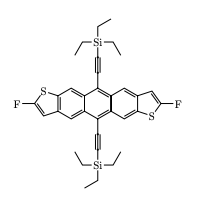
\includegraphics{img/adt-tes-f.png}
    \caption[Molecular diagram of ADT TES-F.]{Molecular diagram of fluorinated anthradithiophene (ADT) with triethylsilyethynyl (TES) side group. A drop-cast sample of this molecule was provided by the Ostroverkhova group at Oregon State University, and used for demonstration of our microspectrometer instrument following a study by Lam \cite{lam_polarization_2018}.}
    \label{fig:adt-diagram}
\end{figure}

\subsubsection{Quantum Dots: \ce{CdSe}}\label{chap:intro-optomats-qd}

Quantum dots (QDs) are artificial semiconductor particles, typically only a few nanometers in size. There has been a fair amount of research on the tunability of optoelectronic properties in QDs by varying their size and shape. Quantum dots have many of the same potential applications as other optoelectronic materials but are attractive for their size and reproducibility. Previous studies have shown how quantum dots can be produced en masse with a high degree of control over their shape and size \cite{empedocles_photoluminescence_1996, murray_synthesis_2000}.

A sample of CdSe quantum dots, suspended in solution and drop-cast on a glass slide, is used to demonstrate the new microspectrometer device in Chapter \ref{chap:results}.

\subsection{Mechanics of Photoluminescence}
Photoluminescence occurs in molecules where the valence and conduction bands are separated by a small band gap near the Fermi level. A molecule absorbs a photon with energy greater than or equal to its band gap, exciting an electron from its ground state in the valence band to an excited state in the conduction band. The electron lives in this excited state for a short time, and then relaxes back to the ground state.

The electron can relax non-radiatively --- losing energy as it transitions through vibrational modes --- or radiatively, losing a small amount of energy to vibrational transitions and then returning to the ground state. When it returns to the ground state, the energy is emitted as a photon. \hl{We expect the energy of this photon to be lower than that of the absorbed photon (and the wavelength longer) because of the loss of energy to vibrational transitions.}

% Because of the loss of energy to vibrational transitions, we expect the energy of this photon to be lower than that of the absorbed photon, and the wavelength longer.

Measurement of fluorescent emissions yields information about the energy of these electron transitions, allowing us to map out the electron band structure of molecules.
